\mode*
\section{Optimierung}

%%%%%%%%%%%%%%%%%%%%%%%%%%%%%%%%%%%%%%%%%%%%%%%%%%%%%%%%%%%% 
%%%%%%%%%%%%%%%%%%%%%%%%%%%%%%%%%%%%%%%%%%%%%%%%%%%%%%%%%%%%
\subsection{Lagrange-Multiplikatoren}

\begin{frame}{Minimierung mit Nebenbedingungen}
  Aufgabe dieses Abschnitts: finde $\vx^* \in \R^n$, so dass
  \begin{gather*}
    f(\vx)
  \end{gather*}
  minimiert wird, unter der Nebenbedingung, dass
  \begin{gather*}
    g(\vx^*)=0 
  \end{gather*}
  gilt. Analog kann natürlich auch maximiert werden.
\end{frame}

%%%%%%%%%%%%%%%%%%%%%%%%%%%%%%%%%%%%%%%%%%%%%%%%%%%%%
\begin{frame}
  \frametitle{Einfaches Beispiel}  
  \begin{itemize}
  \item Wir suchen den/die Punkt(e) auf der Hyperbel $xy=3$, der/die am nächsten am Ursprung liegt
  \end{itemize}
  \begin{center}
    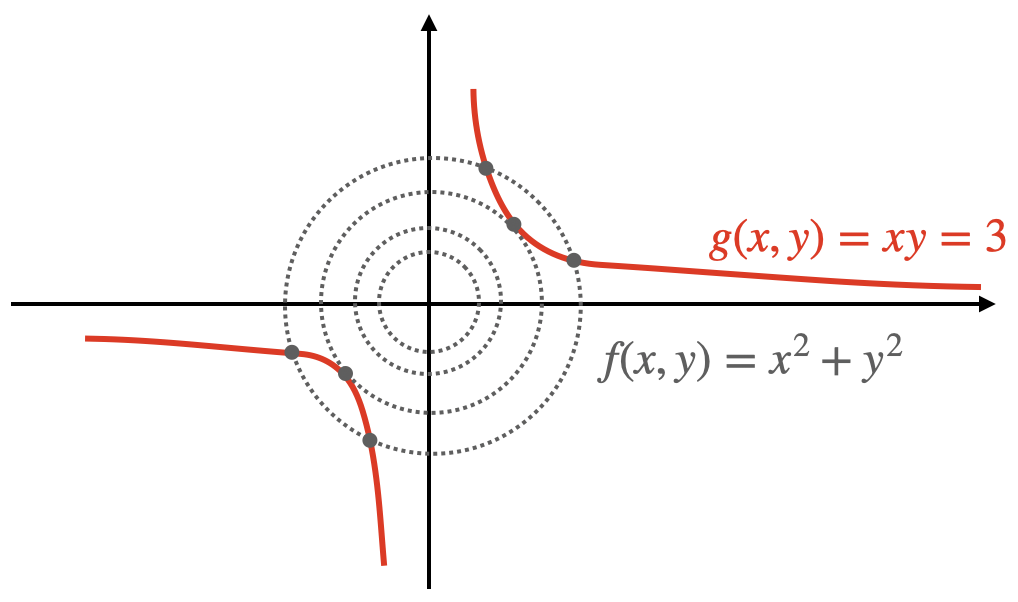
\includegraphics[width=0.7\textwidth]{img/mv22.png}
  \end{center}
  
  \begin{itemize}
  \item Geometrische Lösung: Berührungspunkt vom kleinstmöglichen Kreis um den Ursprung und der Hyperbel
  \end{itemize}
\end{frame}

\begin{frame}
  \frametitle<presentation>{Einfaches Beispiel: mathematische Formulierung}
  Finde das $\vx^*=(x,y)$, so dass
  \begin{gather*}
    f(\vx) = x^2+y^2
  \end{gather*}
  minimal ist, und die Nebenbedingung
  \begin{gather*}
    g(\vx^*) = xy -3 = 0
  \end{gather*}
  gilt.
  \begin{itemize}
  \item Die Wurzelfunktion ist monoton, wir können also das Quadrat minimieren.
  \end{itemize}
\end{frame}

\begin{frame}
  \frametitle<presentation>{Einfaches Beispiel: Eigenschaften}
  \begin{center}
    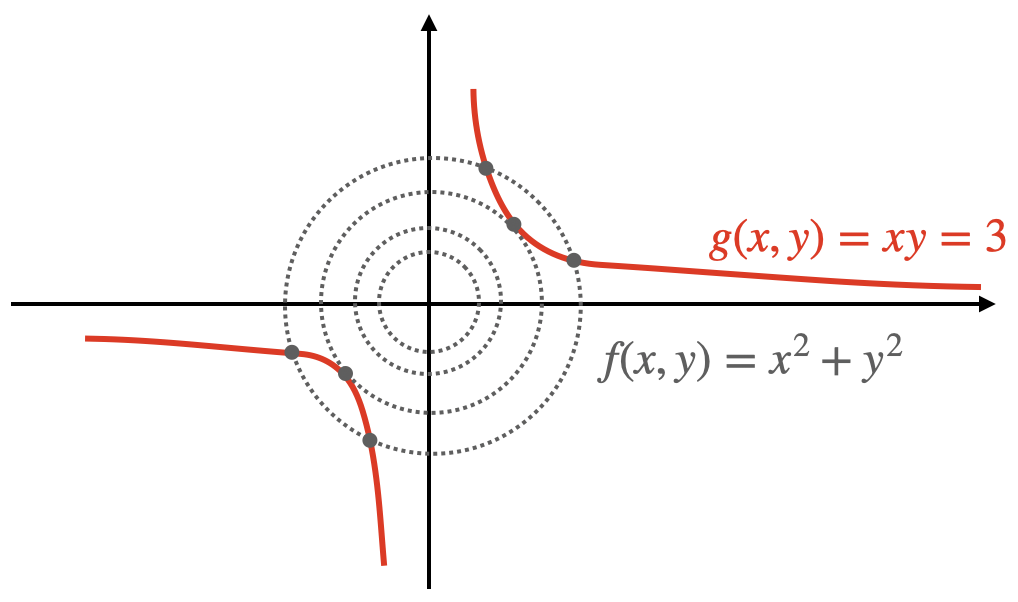
\includegraphics[width=0.6\textwidth]{img/mv22.png}
  \end{center}

  \begin{itemize}
  \item Die Eigenschaft $\nabla f=0$ gilt nur im Ursprung, ist also hier nicht anwendbar
  \item Parametrisiere die Kurve $xy-3=0$ mit $\vx(t)$,
    so dass $\vx^*=\vx(0)$
  \item Dort gilt die eindimensionale Minimalbedingung
    \begin{gather*}
      d_t f(\vx(0)) = \nabla f(\vx(0))\cdot \vx'(0) = 0
    \end{gather*}
  \end{itemize}
\end{frame}

%%%%%%%%%%%%%%%%%%%%%%%%%%%%%%%%%%%%%%%%%%%%%%%%%%%%%%%%%%%%
\begin{frame}
  \frametitle<presentation>{Einfaches Beispiel: Lagrange-Multiplikator}
  \begin{center}
    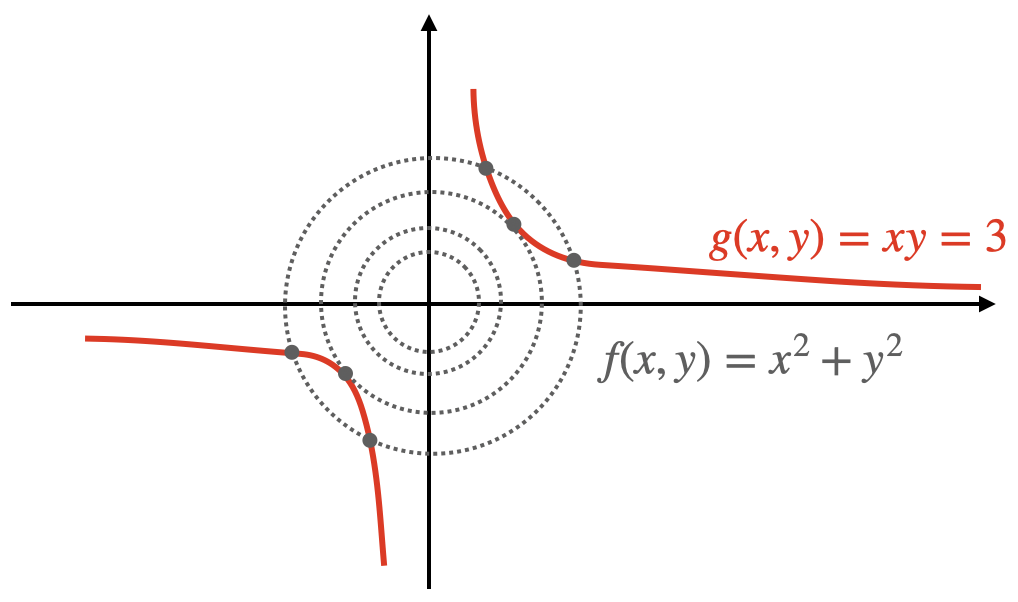
\includegraphics[width=0.6\textwidth]{img/mv22.png}
  \end{center}
  
  \begin{itemize}
  \item Es ist also der Tangentialvektor von $\vx(t)$ orthogonal zu $\nabla f$.
  \item Der Tangentialvektor einer Kurve ist auch orthogonal zum Gradienten (s. Kap. 2)
  \item Es ist also $\nabla f(\vx^*)$ parallel zu $\nabla g(\vx^*)$ und es gibt $\lambda$ mit
    \begin{gather*}
      \nabla f(\vx^*) = \lambda \nabla g(\vx^*)
    \end{gather*}
  \item $\lambda$ heißt \textbf{Lagrange-Multiplikator}
  \end{itemize}  
\end{frame}

\begin{frame}
  \frametitle<presentation>{Einfaches Beispiel: Lagrange-System}
  \begin{itemize}
  \item Wir suchen nun die Lösung $(\vx^*,\lambda)$ des Systems
    \begin{gather*}
      \begin{aligned}
        \nabla f(\vx^*) - \lambda \nabla g(\vx^*) &= 0\\
        g(\vx^*) &=0
      \end{aligned}
      \quad\Leftrightarrow\quad
      \begin{aligned}
      \begin{pmatrix}
        2 & -\lambda\\-\lambda & 2
      \end{pmatrix}
        \begin{pmatrix}
          x^*\\y^*
        \end{pmatrix}
        &= 0\\
          x^*y^*-3 &= 0
      \end{aligned}
    \end{gather*}
  \item Für beliebiges $\lambda$ löst $\vx^*=0$ das LGS, aber nicht die Nebenbedingung
    \only<3->{
    \item Die Matrix muss singulär werden, also
      \begin{itemize}
      \item $\lambda=2$: $x^*=y^*$
      \item $\lambda=-2$: $x^*=-y^*$
      \end{itemize}
    \item Im ersten Fall löst $x^*=y^*=\pm\sqrt{3}$ die Aufgabe.
    \item Im zweiten Fall gibt es keine Lösung, da $xy=3>0$ gelten soll
    }
  \end{itemize}
  \only<2>{
    \begin{Denkpause}
      Wie muss $\lambda$ gewählt werden, damit es weitere Lösungen des LGS gibt?
    \end{Denkpause}
  }
\end{frame}

\begin{frame}{Lagrange-Formalismus}
  \begin{itemize}
  \item Jede Lösung der beschränkten Minimierungsaufgabe ist notwendig
    ein stationärer Punkt der \textbf{Lagrange-Funktion}
    \begin{gather*}
      L(\vx,\lambda) \equiv f(\vx) - \lambda g(\vx)
    \end{gather*}
  \item Die Kandidaten erfüllen damit das Gleichungssystem
    \begin{gather*}
      \nabla L(\vx,\lambda) = 0
      \quad\Leftrightarrow\quad
      \begin{aligned}
        \nabla f(\vx) - \lambda \nabla g(\vx) &= 0\\
        -g(\vx) &=0
      \end{aligned}
    \end{gather*}
  \end{itemize}
  \pause
  \begin{Denkpause}
    Was fehlt?
  \end{Denkpause}
\end{frame}

\begin{frame}{Hinreichende Bedingung}
  \begin{itemize}
  \item Um festzustellen, ob es sich um ein Minimum, Maximum,
    etc. handelt betrachten wir jetzt die Hesse-Matrix
    \begin{gather*}
       H_{L}=\nabla^2_{\vx} L(\vx^*,\lambda) = \nabla^2f(\vx^*) - \lambda \nabla^2 g(\vx^*)
    \end{gather*}
  \item Da nur Punkte mit $g(\vx)=0$ zugelassen sind, sind nur
    Variationen in Richtungen $\vv\perp\nabla g(\vx^*)$ relevant
  \item Ein lokales Minimum genau dann, wenn
    \begin{gather*}
      \nabla L = 0 \quad \wedge \quad
      \vv^TH_{L}\vv \ge 0 \;\forall \vv\perp\nabla g
    \end{gather*}
  \item Ein lokales Maximum genau dann, wenn
    \begin{gather*}
      \nabla L = 0 \quad \wedge \quad
      \vv^TH_{L}\vv \le 0 \;\forall \vv\perp\nabla g
    \end{gather*}
  \end{itemize}
\end{frame}

%%%%%%%%%%%%%%%%%%%%%%%%%%%%%%%%%%%%%%%%%%%%%%%%%%%%%%%%%%%%
\begin{frame}{Beispiel: Oberflächenminimierung}
  \begin{itemize}
  \item Ein stabförmiges Bakterium möchte seine Oberfläche minimieren
  \item Es sei der Einfachheit halber zylinderförmig angenommen
    \begin{itemize}
    \item $h$ Höhe
    \item $r$ Radius
    \end{itemize}
  \item Sein Volumen ist fest: $V = \pi r^2h = V_0$
  \item Die Oberfläche ist $A=2\pi r^2+2\pi r h$
    \begin{itemize}
    \item 2 Deckel je $\pi r^2$
    \item Mantel $2\pi r h$
    \end{itemize}
  \item Die Lagrange-Funktion lautet
    \begin{gather*}
      L(r,h,\lambda) = 2\pi r^2+2\pi r h - \lambda(\pi r^2h - V_0)
    \end{gather*}
  \end{itemize}
\end{frame}

%%%%%%%%%%%%%%%%%%%%%%%%%%%%%%%%%%%%%%%%%%%%%%%%%%%%%%%%%%%%
\begin{frame}
  \frametitle<presentation>{Oberflächenminimierung: kritische Punkte}
  \begin{itemize}
  \item Zunächst:
    \begin{align*}
      0=\partial_r L &= 4\pi r + 2\pi h - 2\lambda \pi rh\\
      0=\partial_h L &= 2\pi r - \lambda \pi r^2
    \end{align*}
  \item Die zweite Gleichung impliziert sofort $\lambda = 2/r$
    \pause
  \item Einsetzen in die erste:
    \begin{gather*}
      0=4\pi r+ 2\pi h - 4 \pi h
      \qquad\Rightarrow\qquad h=2r
    \end{gather*}
  \item Aus der Nebenbedingung bekommen wir
    \begin{gather*}
      V = \pi r^2 h = 2\pi r^3 = V_0
      \quad\Rightarrow\quad r = \sqrt[3]{\frac{V_0}{2\pi}}
    \end{gather*}
  \end{itemize}
\end{frame}

%%%%%%%%%%%%%%%%%%%%%%%%%%%%%%%%%%%%%%%%%%%%%%%%%%%%%%%%%%%%
\begin{frame}
  \frametitle<presentation>{Oberflächenminimierung: Hesse-Matrix}
  \begin{itemize}
  \item Die Hesse-Matrix lautet
    \begin{gather*}
      H_L =
      \begin{pmatrix}
        \partial_{rr} L & \partial_{rh} L\\
        \partial_{hr} L & \partial_{hh} L
      \end{pmatrix}
      = 2\pi
      \begin{pmatrix}
        2-\lambda h & 1-\lambda r\\
        1-\lambda r & 0
      \end{pmatrix}
    \end{gather*}
  \item Einsetzen von $\lambda=2/r$ und $h=2r$ ergibt
    \begin{gather*}
      H_L =
      \begin{pmatrix}
        -4\pi & -2\pi\\
        -2\pi & 0
      \end{pmatrix}
    \end{gather*}
  \item Als nächstes benötigen wir $\nabla g$ \visible<2->{{\color{blue}für $h=2r$}}.
    \begin{gather*}
      \partial_r g = 2\pi r h \visible<2->{{\color{blue}=4\pi r^2}}
      \quad \partial_h g = \pi r^2
      \visible<2->{{\color{blue}\qquad\nabla g = \pi r^2
          \begin{pmatrix}
            4\\1
          \end{pmatrix}
        }}
    \end{gather*}
  \item<2-> Damit erfüllen Vektoren $\vv\perp\nabla g$ die Gleichung $v_2 = -4v_1$
  \end{itemize}
\end{frame}

%%%%%%%%%%%%%%%%%%%%%%%%%%%%%%%%%%%%%%%%%%%%%%%%%%%%%%%%%%%%
\begin{frame}
  \frametitle<presentation>{Oberflächenminimierung: Definitheit}
  \begin{gather*}
    H_L =
    \begin{pmatrix}
      -4\pi & -2\pi\\
      -2\pi & 0
    \end{pmatrix}
  \end{gather*}
  \begin{itemize}
  \item Es genügt, den Vektor $\vv=(1,-4)$ einzusetzen. (Warum?)
    \begin{gather*}
      \vv^T H_L\vv = (1,-4)
      \begin{pmatrix}
        -4\pi + 8\pi\\-2\pi
      \end{pmatrix}
      = 12\pi > 0
    \end{gather*}
  \item Es handelt sich also um ein Minimum
  \end{itemize}
\end{frame}

%%%%%%%%%%%%%%%%%%%%%%%%%%%%%%%%%%%%%%%%%%%%%%%%%%%%%%%%%%%%
\begin{frame}
  \frametitle<presentation>{Oberflächenminimierung: Bemerkung}
  \begin{itemize}
  \item Berechnen wir $\vv^TH_L\vv$ mit $\vv$ parallel zu $\nabla g$, erhalten wir
    \begin{gather*}
      (4,1)
      \begin{pmatrix}
        -4\pi & -2\pi\\
        -2\pi & 0
      \end{pmatrix}
      \begin{pmatrix}
        4\\1
      \end{pmatrix}
      = (4,1)
      \begin{pmatrix}
        -16\pi -2\pi\\-8\pi
      \end{pmatrix}
      = -80 \pi < 0
    \end{gather*}
    \begin{itemize}
    \item Die Matrix $H_L$ ist also auf dem gesamten Raum $\R^2$ indefinit
    \item Relevant ist aber nur $\vv\perp\nabla g$
    \end{itemize}
  \end{itemize}
\end{frame}

%%%%%%%%%%%%%%%%%%%%%%%%%%%%%%%%%%%%%%%%%%%%%%%%%%%%%%%%%%%%
\begin{frame}{Zur Bedeutung des Lagrange-Multiplikators}
  \begin{itemize}
  \item Wir kürzen ab: $L(V,\lambda) = A(V) - \lambda (V-V_0)$
  \item Sei nun $A(V)$ zu jedem $V$ die optimale Fläche, also
    \begin{gather*}
      \nabla L(A(V),\lambda) =
      \begin{pmatrix}
        \partial_V A - \lambda\\
        V-V_0
      \end{pmatrix}
      = 0.
    \end{gather*}
  \item Es gilt also $\lambda = \partial_V A$
  \item Der Lagrange-Multiplikator gibt an, wie sich das Optimum
    verändert, wenn ich die Nebenbedingung variiere
  \end{itemize}
\end{frame}

%%%%%%%%%%%%%%%%%%%%%%%%%%%%%%%%%%%%%%%%%%%%%%%%%%%%%%%%%%%% 
\begin{frame}{Beispiel in drei Dimensionen}
  \begin{itemize}
  \item Finde das Minimum der Funktion
  \begin{gather*}
    f(\vx) \equiv f(x,y,z) = 2x-y+z
  \end{gather*}
  unter der Nebenbedingung
  \begin{gather*}
    g(\vx)\equiv x^2+y^2+z^2-1 = 0
  \end{gather*}
  \item Wir stellen zunächst den Gradienten der Lagrange-Funktion auf
    \begin{gather*}
      \nabla L (\vx,\lambda) =
      \begin{pmatrix}
       \partial_x L (x,y,z,\lambda)\\
       \partial_y L (x,y,z,\lambda)\\
       \partial_z L (x,y,z,\lambda)\\
       \partial_\lambda L (x,y,z,\lambda)
      \end{pmatrix}
      =
      \begin{pmatrix}
        2-2\lambda x\\
        -1-2\lambda y\\
        1-2\lambda z\\
        x^2+y^2+z^2-1
      \end{pmatrix}
      \stackrel!= 0
    \end{gather*}
  \end{itemize}
\end{frame}

\begin{frame}
  \frametitle<presentation>{Beispiel in drei Dimensionen: Rechnung}
  \begin{itemize}
  \item Die drei ersten Gleichungen lassen sich nach $x,y,z$ auflösen
    \begin{gather*}
      x = \frac1\lambda,\qquad y = \frac{-1}{2\lambda},\qquad
      z=\frac1{2\lambda}
    \end{gather*}
  \item Dies setzen wir in die Nebenbedingung ein
    \begin{gather*}
      x^2+y^2+z^2 = \frac1{\lambda^2}+\frac1{4\lambda^2}+\frac1{4\lambda^2}
      = \frac3{2\lambda^2}
      \stackrel!= 1,
    \end{gather*}
    was $\lambda^2=3/2$ ergibt.
  \end{itemize}
  \pause
  \begin{Denkpause}
    Warum erwarten wir zwei Lösungen?
  \end{Denkpause}
\end{frame}

\begin{frame}
  \frametitle<presentation>{Beispiel in drei Dimensionen: Einsetzen}
  \begin{itemize}
  \item Setzen wir nun $\lambda = \pm \sqrt{3/2}$ in die Gleichungen der
    anderen Variablen ein, erhalten wir zwei Punkte
    \begin{gather*}
      \vx_1 = \left(\frac2{\sqrt{6}},\frac{-1}{\sqrt6},\frac{1}{\sqrt6}\right),
      \qquad
      \vx_1 = \left(-\frac2{\sqrt{6}},\frac{1}{\sqrt6},\frac{-1}{\sqrt6}\right)
    \end{gather*}
  \item In diesem Fall ist die Hesse-Matrix $\nabla^2f=0$. Aber:
    \begin{gather*}
      H_L =
      \begin{pmatrix}
        0 & 0 & 0\\
        0 & 0 & 0\\
        0 & 0 & 0
      \end{pmatrix}
      -\lambda
      \begin{pmatrix}
        2 &&\\&2&\\&&2
      \end{pmatrix}
    \end{gather*}
  \item Damit erhalten wir:
    \begin{itemize}
    \item $\lambda = +\sqrt{3/2}$: $\vx_1$ Maximum, $f(\vx_1) = \sqrt6$
    \item $\lambda = -\sqrt{3/2}$: $\vx_2$ Minimum, $f(\vx_2) = -\sqrt6$
    \end{itemize}
  \end{itemize}
\end{frame}

%%%%%%%%%%%%%%%%%%%%%%%%%%%%%%%%%%%%%%%%%%%%%%%%%%%%%%%%%%%%
\begin{frame}{Abschlussfragen}
  \begin{enumerate}
  \item Warum führen wir Langrange-Multiplikatoren ein?
  \item Was wissen wir über die Gradienten der zu minimierenden
    Funktion und der Nebenbedingung im Optimum?
  \item Was ist die Lagrange-Funktion und wie finden wir mit ihr
    kritische Punkte?
  \item Wie ist die Darstellung der verwendeten Hesse-Matrix?
  \item Wie unterscheidet sich die hinreichende Bedingung an Extrema
    vom unbeschränkten Fall?
  \end{enumerate}
\end{frame}

%%%%%%%%%%%%%%%%%%%%%%%%%%%%%%%%%%%%%%%%%%%%%%%%%%%%%%%%%%%%
%%%%%%%%%%%%%%%%%%%%%%%%%%%%%%%%%%%%%%%%%%%%%%%%%%%%%%%%%%%%
\subsection{Steilster Abstieg (gradient descent)}
%%%%%%%%%%%%%%%%%%%%%%%%%%%%%%%%%%%%%%%%%%%%%%%%%%%%%%%%%%%%
\begin{frame}{Wie findet man Minima?}
  Bleiben wir beim Bild der Wanderung
  \only<1>{
    \begin{Denkpause}
      Sie stehen an einem Hang und wollen die Talsohle erreichen. In
      welche Richtung gehen Sie?
    \end{Denkpause}
  }
  \pause
  \begin{itemize}
  \item Nach unten!
  \item Am schnellsten abwärts geht es in Richtung
    \begin{gather*}
      -\nabla f
    \end{gather*}
  \item Das ist die \textbf{Richtung des steilsten Abstiegs}
  \item Daraus leitet sich das \textbf{Verfahren des steilsten
      Abstiegs}, auf Englisch \textbf{gradient descent} ab.
  \item Es wird eingesetzt zur Minimierung, z.B. einer Energie
  \item In der Sprache der Optimierung minimieren wir eine
    \textbf{Kostenfunktion}
  \end{itemize}
\end{frame}

%%%%%%%%%%%%%%%%%%%%%%%%%%%%%%%%%%%%%%%%%%%%%%%%%%%%%%%%%%%%
\begin{frame}{Definition des Verfahrens des steilsten Abstiegs}
  Gradient descent
  \begin{itemize}
  \item Ausgehend von einem \textbf{Startwert} $\vx_0$ generiert das
    Verfahren eine Folge
    \begin{gather*}
      \vx_1,\vx_2,\ldots
    \end{gather*}
    mit dem Ziel, sich dem Minimum anzunähern.
  \item Sei $f(\vx)$ die Kostenfunktion
  \item Nach $n$ Schritten des Verfahrens berechnen wir $\vx_{n+1}$ durch
    \begin{gather*}
      \vx_{n+1} = \vx_{n} - \eta \nabla f(\vx_{n})
    \end{gather*}
  \item $\eta$ ist die \textbf{Lernrate} oder auch \textbf{Schrittweite}
  \end{itemize}
\end{frame}


%%%%%%%%%%%%%%%%%%%%%%%%%%%%%%%%%%%%%%%%%%%%%%%%%%%%%%%%%%%%
\begin{frame}{Beispiel}
  \begin{gather*}
    f(x,y) = x^2+2y^2+2\sin(xy)
    \qquad
    \nabla f(x,y) = \begin{pmatrix}2x+2y\cos(xy) \\ 4y+2x\cos(xy)\end{pmatrix}
  \end{gather*}
  \begin{itemize}
  \item Startpunkt: $(x_0,y_0) = (1,2)$
  \item Lernrate: $\eta=0.1$
  \item Iteration:
    \begin{center}
      \begin{tabular}[b]{c|rr}
        Schritt & $x$ & $y$ \\\hline
        $\vx_0$ & 1.0000 & 2.0000 \\
        $\vx_1$ & 0.9665 & 1.2832 \\
        $\vx_2$ & 0.6899 & 0.7072 \\
        $\vx_3$ & 0.4269 & 0.3024 \\
        $\vx_4$ & 0.2816 & 0.0968 \\
        \vdots & \vdots & \vdots\\
        $\vx_{100}$ & 0.0001 & -0.0001
      \end{tabular}
      \includegraphics[width=.25\textwidth]{fig/steepest.tikz}
    \end{center}
  \end{itemize}
\end{frame}

%%%%%%%%%%%%%%%%%%%%%%%%%%%%%%%%%%%%%%%%%%%%%%%%%%%%%%%%%%%%
\begin{frame}{Abbruchkriterien}
  Das Verfahren läuft undendlich weiter, was aber nicht praktikabel
  ist. Wir können es stoppen, wenn
  \begin{itemize}
  \item Der Gradient klein ist,
    \begin{gather*}
      \left|\nabla f(\vx_n)\right| < \varepsilon
    \end{gather*}
    \begin{itemize}
    \item Äquivalent zu Schrittweite klein:
      \begin{gather*}
        |\vx_{n+1}- \vx_n| < \eta \varepsilon
      \end{gather*}
    \end{itemize}
  \item Maximale Schrittzahl erreicht $n=n_{\text{max}}$
    \begin{itemize}
    \item Nothalt, damit das Programm nicht hängen bleibt
    \end{itemize}
  \item Falls der minimale Wert $f_{\text{min}}$ von $f$ bekannt ist
    \begin{gather*}
      f(\vx_{n}) - f_{\text{min}} < \varepsilon
    \end{gather*}
    \begin{itemize}
    \item Zum Beispiel bei der Nullstellensuche
    \end{itemize}
  \end{itemize}
\end{frame}

%%%%%%%%%%%%%%%%%%%%%%%%%%%%%%%%%%%%%%%%%%%%%%%%%%%%%
\begin{frame}
  \begin{gather*}
    f(x,y) = x^2+2y^2+2\sin(xy)\qquad
    \nabla f(x,y) = \begin{pmatrix}2x+2y\cos(xy) \\ 4y+2x\cos(xy)\end{pmatrix}
  \end{gather*}
  
\centerline{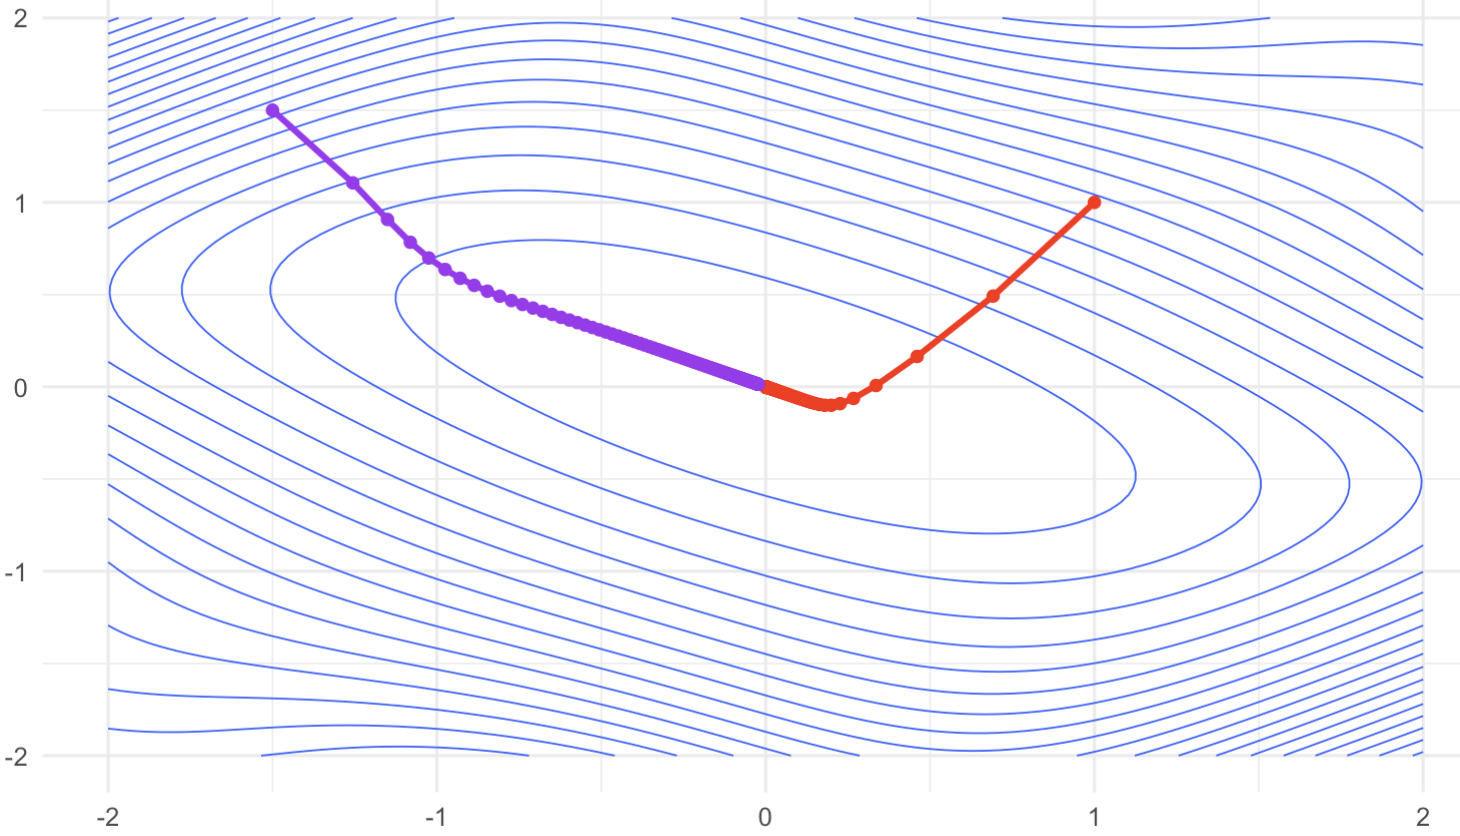
\includegraphics[width=.9\textwidth]{img/gd1.png}}
\end{frame}

%%%%%%%%%%%%%%%%%%%%%%%%%%%%%%%%%%%%%%%%%%%%%%%%%%%%%
\begin{frame}
    \frametitle{Wahl des Startpunkts}
    \begin{itemize}
        \item Konvergenz hängt vom {\bf Startpunkt} ab
          \begin{itemize}
            \item Kann viele Iterationsschritte benötigen
            \item Kann in ein lokales Minimum führen
            \item Kann in einen Sattelpunkt führen (unwahrscheinlich)
        \end{itemize}
    \end{itemize}

    \centerline{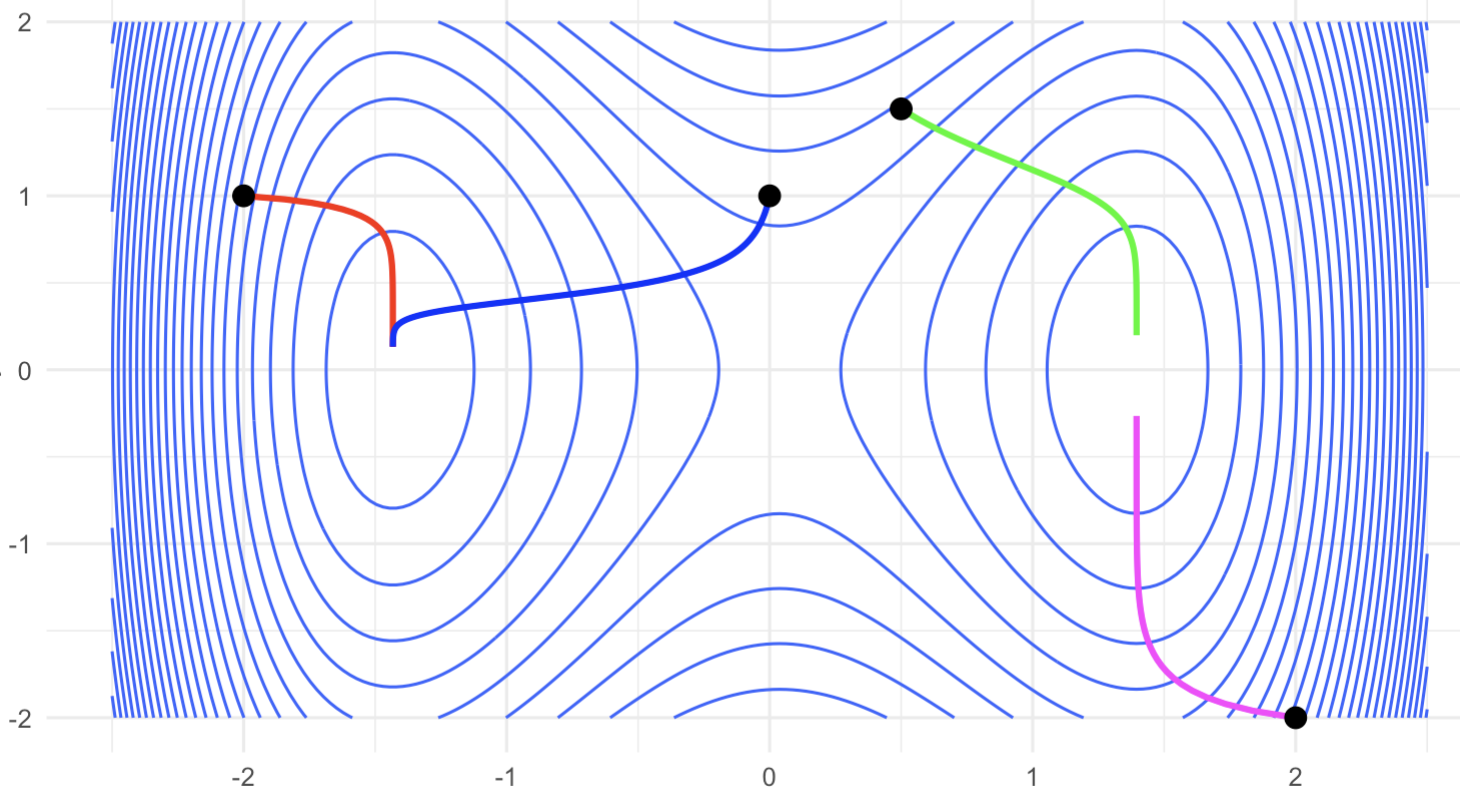
\includegraphics[width=.8\textwidth]{img/gd3.png}}
    \begin{itemize}
        \item Mögliche Strategien: zufällige, mehrfache Startpunkte; benutzen von Vorwissen; ...
    \end{itemize}
\end{frame}



%%%%%%%%%%%%%%%%%%%%%%%%%%%%%%%%%%%%%%%%%%%%%%%%%%%%% 
\begin{frame}
    \frametitle{Lokale und globale Minima}
    \begin{itemize}
        \item GD konvergiert zu einem {\bf lokalen Minimum}!
            \item Lokales Minimum: $f(x) \ge f(x_0)$ für alle $x$ in einer Umgebung von $x_0$.
            \item Globales Minimum: $f(x) \ge f(x_0)$ für alle $x$ im Definitionsbereich.
        \item Meistens suchen wir jedoch das {\bf globale Minimum}
    \end{itemize}
\centerline{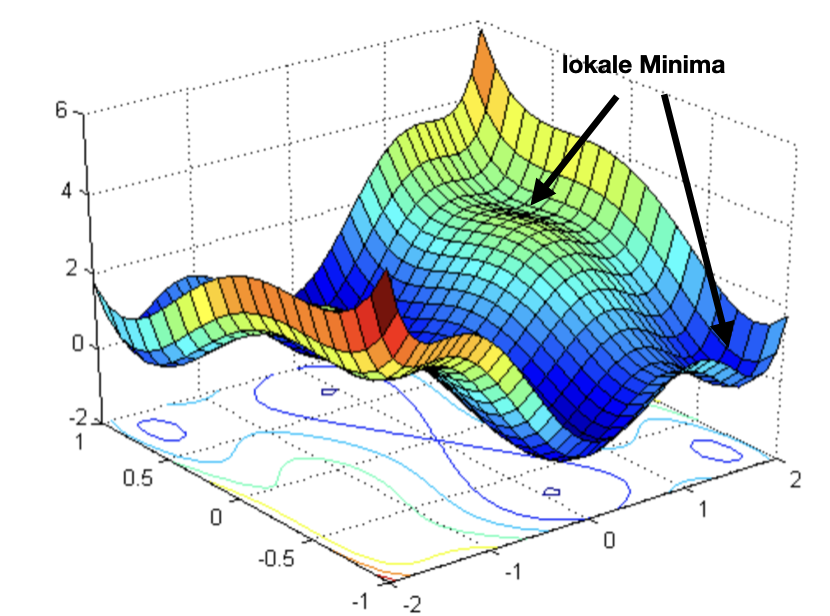
\includegraphics[width=.6\textwidth]{img/local.png}}

\end{frame}


%%%%%%%%%%%%%%%%%%%%%%%%%%%%%%%%%%%%%%%%%%%%%%%%%%%%%
\begin{frame}
    \frametitle{Konvexe Funktionen}
    \begin{itemize}
        \item Eine Funktion $f$ ist {\bf konvex}, wenn für alle $p_1, p_2 \in \mathbb{R}^n$ im Definitionsbereich gilt:
        $$
        f(\lambda p_1 + (1-\lambda)p_2) \leq \lambda f(p_1) + (1-\lambda)f(p_2)~~~~~\forall \lambda \in [0,1]
        $$
        \item anders gesagt: verbindet man 2 Punkte auf der Fläche, dann ist die Verbindungslinie immer oberhalb der Fläche.
        \item Besitzt eine konvexe Funktion ein Minimum, dann ist es immer ein {\bf globales Minimum}: bei den Funktionen funktioniert GD besonders zuverlässig!
        \item Beispiel: $f(x,y) = x^2 + 2y^2$ ist konvex.
    \end{itemize}

\end{frame}

%%%%%%%%%%%%%%%%%%%%%%%%%%%%%%%%%%%%%%%%%%%%%%%%%%%%%
\begin{frame}
    \frametitle{Wahl der Lernrate}
    
    \begin{itemize}
    \item Das Bild der Wanderung hinkt
      \begin{itemize}
      \item Wir folgen dem Gradienten nicht stetig
      \item Wir teleportieren abhängig von der Lernrate
      \end{itemize}
      \only<1>{
        \begin{Denkpause}
          Was kann dadurch schiefgehen?
        \end{Denkpause}
      }
      \pause
    \item Wahl der Lernrate $\eta$ entscheidend
      \begin{itemize}
      \item Zu klein: langsame Konvergenz
      \item Zu groß: divergiert, springt über Minimum
      \end{itemize}
    \end{itemize}
    \centerline{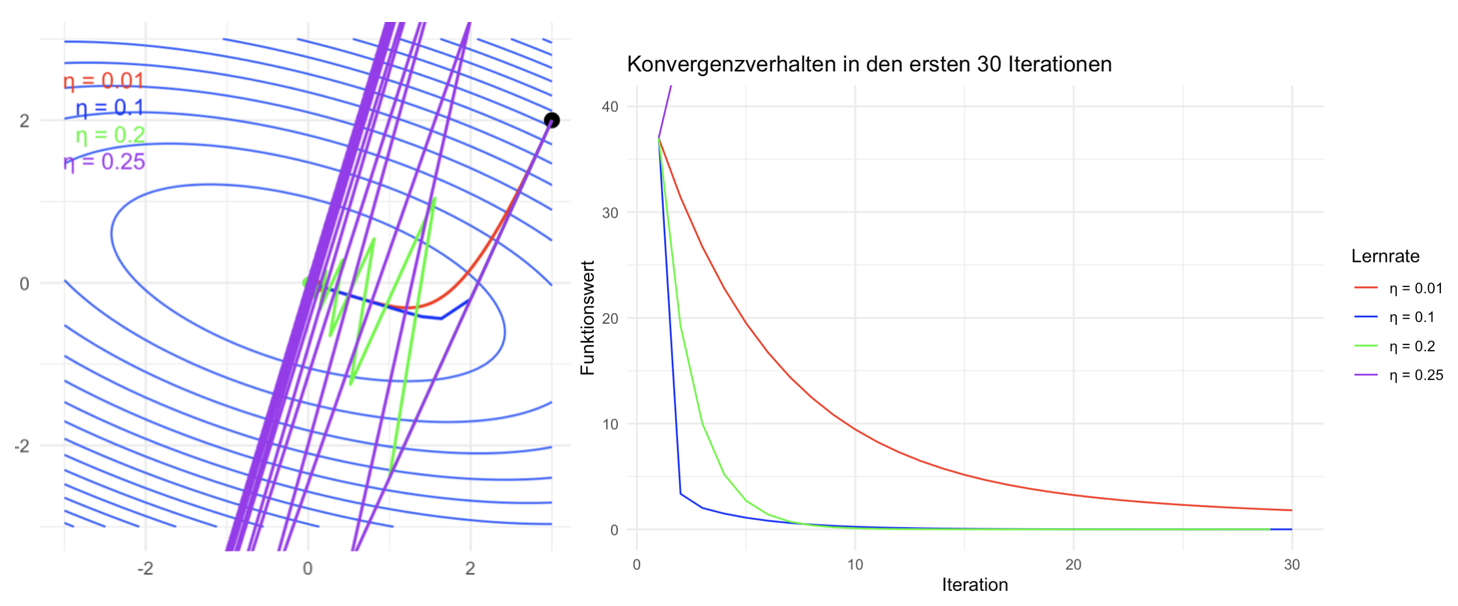
\includegraphics[width=1.1\textwidth]{img/gd4.png}}
\end{frame}

%%%%%%%%%%%%%%%%%%%%%%%%%%%%%%%%%%%%%%%%%%%%%%%%%%%%%
\begin{frame}{Strategien für die Lernrate}
  \begin{itemize}
  \item \glqq{}Schrittweitenhalbierung\grqq{} mit gewählter Grundschrittweite $\eta$
    \begin{enumerate}
    \item Berechne $\vd_n = -\eta\nabla f(\vx_n)$
    \item Berechne $f(\vx_n+\vd_n)$
    \item Ist dieser Wert größer als $f(\vx_n)$, halbiere $\vd_n$ und gehe zu 2.
      \begin{itemize}
      \item Hintergrund: wenn wir minimieren ist es nicht sinnvoll zu
        größeren Werten zu gehen
      \item Achtung! Die Gefahr in einem lokalen Minimum steckenzubleiben wächst
      \end{itemize}
    \end{enumerate}
  \item Line search
    \begin{enumerate}
    \item Betrachte die Funktion $g(t) = f(\vx_n-t\nabla f(\vx_n))$
    \item Finde deren Minimum für $t>0$
      \begin{itemize}
      \item Eindimensionale Minimierung ist einfacher!
      \end{itemize}
      \item Wähle dieses $t$ als Schrittweite $\eta$
    \end{enumerate}
  \end{itemize}
\end{frame}

%%%%%%%%%%%%%%%%%%%%%%%%%%%%%%%%%%%%%%%%%%%%%%%%%%%%%
\begin{frame}
    \frametitle{Anwendungen in der Bioinformatik}

    \begin{itemize}
        \item Proteinfaltungsvorhersage:
        \begin{itemize}
        \item Finden der energetisch günstigsten Konformation
        \item Die Energielandschaft hat viele lokale Minima
        \item Gradientenabstieg mit stochastischen Komponenten
        \end{itemize}
         \item Molekulardynamik-Simulationen:\
        \begin{itemize}
            \item Energieminimierung von Molekülstrukturen
            \item Berechnung stabiler Konformationen von Biomolekülen
        \end{itemize}        
        \item Machine Learning in der Genomik:
        \begin{itemize}
        \item Training von neuronalen Netzen zur Klassifizierung von Tumor-Subtypen anhand von Genexpressionsdaten.
        \item Vorhersage von Protein-Protein-Interaktionen
        \end{itemize}
    \end{itemize}
\end{frame}

%%%%%%%%%%%%%%%%%%%%%%%%%%%%%%%%%%%%%%%%%%%%%%%%%%%%%%%%%%%%
\begin{frame}{Abschlussfragen}
  \begin{enumerate}
  \item Was ist das Prinzip des Abstiegsverfahrens?
  \item Wo liegt das Problem mit lokalen Minima?
  \item Wo liegt das Problem mit der Lernrate?
  \item Wie wählen Sie den Startwert (Startpunkt)?
  \end{enumerate}
\end{frame}

